\documentclass[11pt,a4paper]{article}
\usepackage[utf8]{inputenc}
\usepackage[margin=1in]{geometry}
\usepackage{graphicx}
\usepackage{hyperref}
\usepackage{xcolor}

\begin{document}
\noindent\textbf{\Large Tech Nation Visa - Exceptional Promise}\\
\noindent\textbf{Criteria:} Mandatory Criteria (Technical Leadership / Innovation)\\
\noindent\textbf{Applicant:} Odeyemi Olusegun Israel\\
\rule{\textwidth}{0.4pt}

\vspace{0.5cm}
\begin{center}
    \textbf{\Large MC-2: Sustained Technical Contributions --- GitHub Repository and Codebase Authorship}
\end{center}
\vspace{0.3cm}

\section*{1. Executive Summary}
I built the AMTTP codebase as the sole author. The public GitHub repository records \textbf{361 commits over eight months} (September 2025 -- April 2026) from my account, covering the full product stack: Python AI services, a TypeScript API gateway and SDKs, a Dart mobile app, Solidity smart contracts, and security/research tooling.

The repository verifies both authorship and delivery: commit history, timestamps, and per-file diffs are public at \texttt{github.com/segetii/AMTTP}. This evidence shows sustained development of a working product across multiple engineering domains.

\section*{2. Development Activity}

\vspace{0.3cm}
\begin{center}
    \fbox{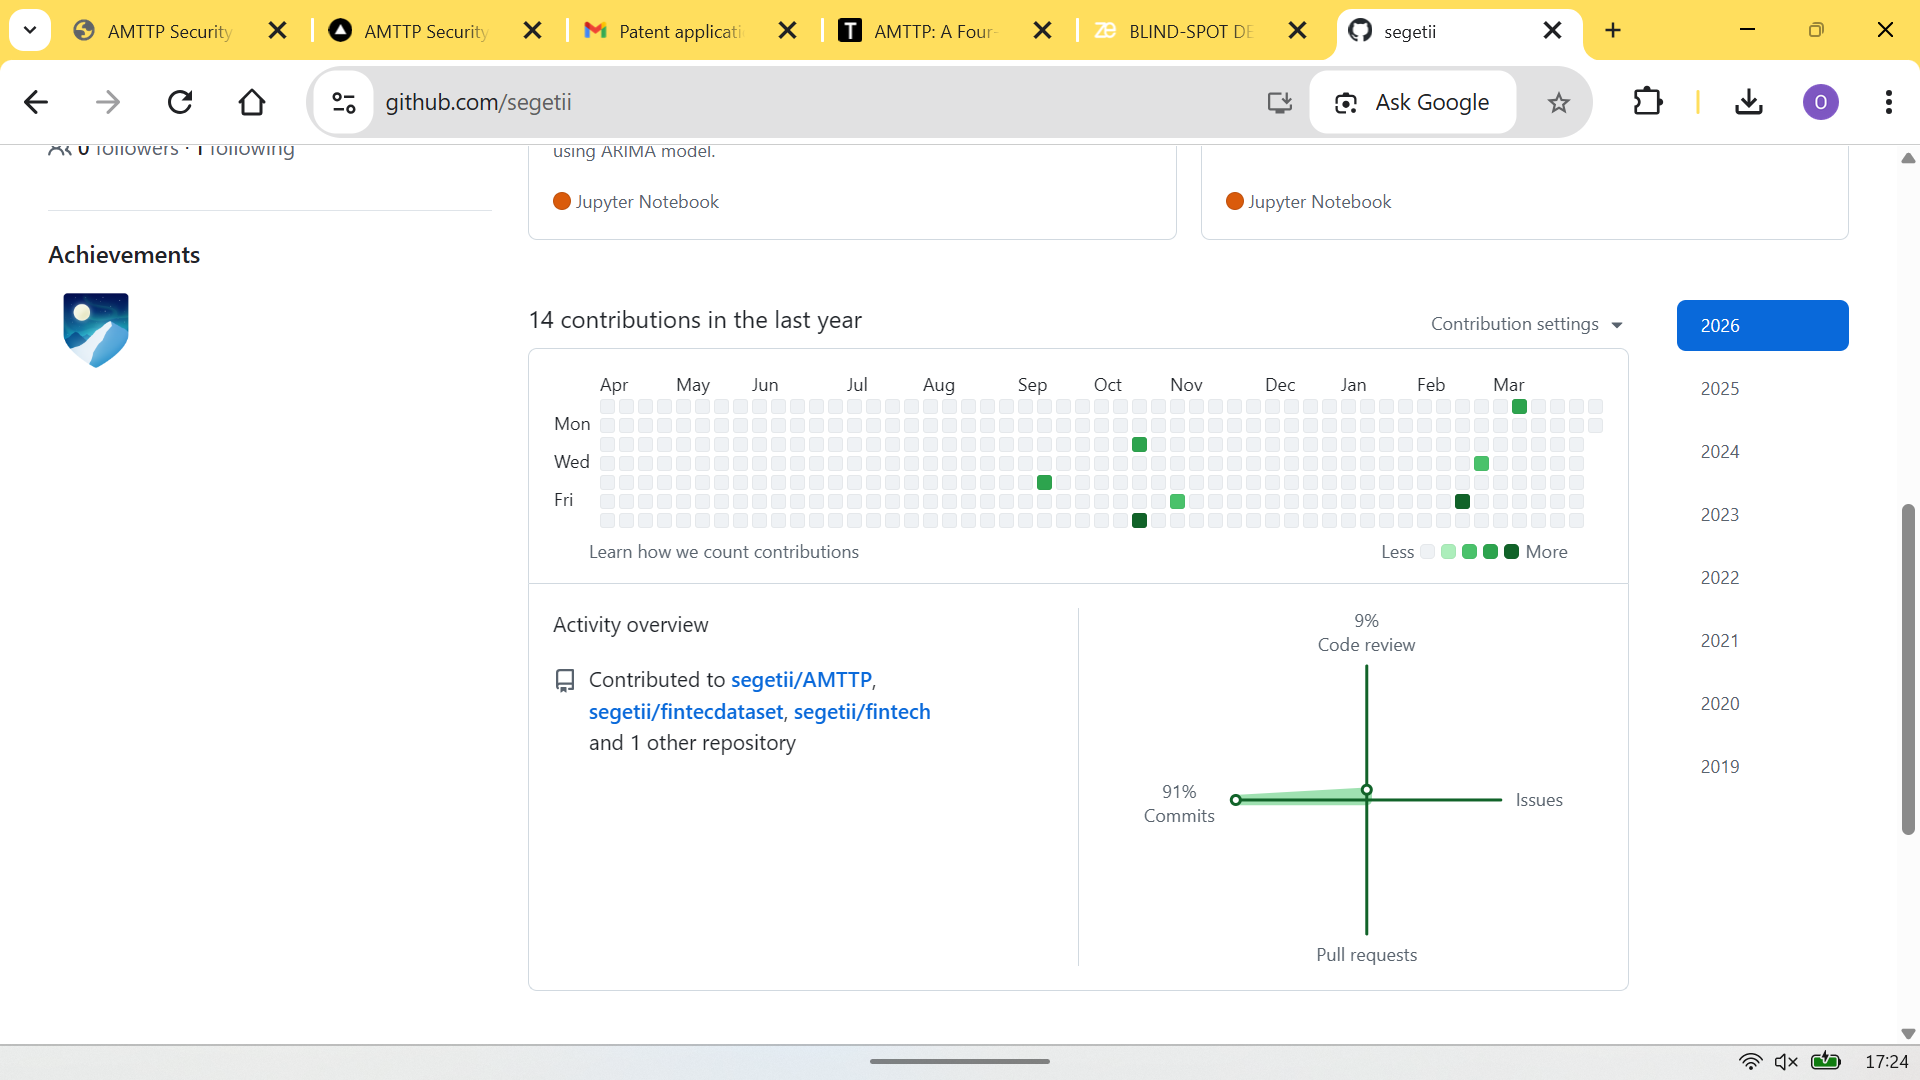
\includegraphics[width=0.88\textwidth]{images/github_green_squares.png}}
\end{center}
\vspace{0.1cm}
\noindent\textit{Figure 1: GitHub activity graph for \texttt{github.com/segetii} --- sustained solo engineering across the full design-to-deployment lifecycle of AMTTP. Each square represents a day with code commits.}

\section*{3. Public Verification Record}
The table below summarises the public development timeline. The volume, cross-domain consistency, and language diversity confirm this is the output of a single senior engineer operating across the full technical stack.

\vspace{0.3cm}
\begin{center}
\begin{tabular}{|l|r|}
\hline
\textbf{Metric} & \textbf{Value} \\
\hline
Total commits (all branches) & 361 \\
Active development period & Sep 2025 -- Apr 2026 \\
Peak month (Mar 2026) & 191 commits \\
Languages & Python, TypeScript, Dart, Solidity \\
Repository & \texttt{github.com/segetii/AMTTP} \\
\hline
\end{tabular}
\end{center}
\vspace{0.1cm}
\textit{Table 1: Public repository summary showing sustained development over eight months in four production languages.}

\vspace{0.3cm}
\noindent\textbf{Development Activity by Month:}
\begin{center}
\begin{tabular}{|l|r|l|}
\hline
\textbf{Month} & \textbf{Commits} & \textbf{Focus} \\
\hline
Sep 2025 & 1 & Project inception \\
Oct 2025 & 22 & Smart contract architecture \\
Nov 2025 & --- & ML model training \& dataset work (Google Colab) \\
Dec 2025 & --- & ML pipeline refinement \& validation (Google Colab) \\
Jan 2026 & 18 & ML pipeline integration \& microservices \\
Feb 2026 & 115 & Full-stack integration \& SDKs \\
Mar 2026 & 191 & Security auditing \& production hardening \\
Apr 2026 & 14 & Research papers \& documentation \\
\hline
\end{tabular}
\end{center}
\vspace{0.1cm}
\textit{Table 2: Monthly cadence (Sep 2025 -- Apr 2026). November and December 2025 commits do not appear in the GitHub graph because ML model training and dataset experimentation during that period were conducted in Google Colab; the resulting model artefacts and pipeline code were pushed to the repository in subsequent months.}

\vspace{0.2cm}
\noindent\textbf{Delivered components:} live public platform at \textbf{amttp.com} (1,220 visitors, 38,320 requests in month 1); complete Solidity contract suite deployed and verified on Ethereum Sepolia; nine-service AI compliance backend; and two developer SDKs enabling third-party integration.

\section*{4. Repository Scope and Authorship}
The repository is a monorepo --- a single codebase that contains every component of the product --- spanning five languages and 14 independently deployable services. Sole authorship across this range --- from Solidity smart contracts to a Flutter mobile app, from ML training pipelines to TypeScript SDKs --- is confirmed at every stage by the public commit history at \texttt{github.com/segetii/AMTTP}.

\vspace{0.3cm}
\noindent\fbox{\begin{minipage}{0.95\textwidth}
\small
\texttt{AMTTP/ (monorepo root)}\\
\texttt{+-- contracts/~~~~~~~~(38 authored Solidity files) UUPS proxy, ZK-NAF, CrossChain}\\
\texttt{+-- backend/~~~~~~~~~(Oracle Gateway + 10 FastAPI microservices)}\\
\texttt{|~~~+-- oracle-service/~~Express.js TypeScript gateway (port 3001)}\\
\texttt{|~~~+-- compliance-service/ orchestrator, sanctions, monitoring}\\
\texttt{+-- ml/~~~~~~~~~~~~~~(XGBoost, LightGBM, GraphSAGE pipelines)}\\
\texttt{|~~~+-- Automation/~~~~risk\_engine/ + ml\_pipeline/ + models/}\\
\texttt{+-- frontend/}\\
\texttt{|~~~+-- frontend/~~~~~~Next.js App Router (War Room, port 3006)}\\
\texttt{|~~~+-- amttp\_app/~~~~~Flutter (6-platform consumer app, port 3010)}\\
\texttt{+-- packages/}\\
\texttt{|~~~+-- client-sdk/~~~~TypeScript SDK (@amttp/client-sdk)}\\
\texttt{|~~~+-- python-sdk/~~~~Python SDK (amttp)}\\
\texttt{+-- research/~~~~~~~~(3 academic papers, visa docs, UDL framework)}\\
\texttt{+-- patents/~~~~~~~~~(8 patent specifications, unified filing)}\\
\texttt{+-- test/~~~~~~~~~~~~(Hardhat + Foundry smart contract tests)}\\
\texttt{+-- audit/~~~~~~~~~~~(Slither + Echidna security pipeline)}
\end{minipage}}
\vspace{0.2cm}

\noindent\textit{Figure 2: Repository directory structure confirming sole authorship across 5 languages and 14+ independently deployable services --- blockchain contracts, ML pipelines, microservices, enterprise dashboard, consumer mobile app, and two developer SDKs, all in one monorepo.}

\vspace{0.3cm}
\noindent\textbf{Repository components:} \texttt{contracts/} (38 original Solidity files), \texttt{ml/} (XGBoost/LightGBM/GraphSAGE pipelines), \texttt{backend/} (10 FastAPI microservices + Express gateway), \texttt{frontend/} (Next.js War Room + Flutter 6-platform app), \texttt{packages/} (TypeScript and Python SDKs for third-party integration).

\vspace{0.3cm}
\noindent\textbf{Technical significance:} Delivering a full-stack compliance platform across blockchain, AI, mobile, and enterprise web demonstrates end-to-end technical ownership. Every commit, timestamp, and per-file diff is permanently public at \texttt{github.com/segetii/AMTTP}; authorship is verifiable without relying on any claim I make.

\vspace{0.4cm}
\noindent\textbf{ML Development Activity (Nov--Dec 2025):} As noted in Table 2, November and December 2025 saw no commits to the public GitHub repository because model training and dataset experimentation were conducted in Google Colab. The Google Drive listing below provides independent, Google-timestamped corroboration.

\vspace{0.2cm}
\begin{center}
    \fbox{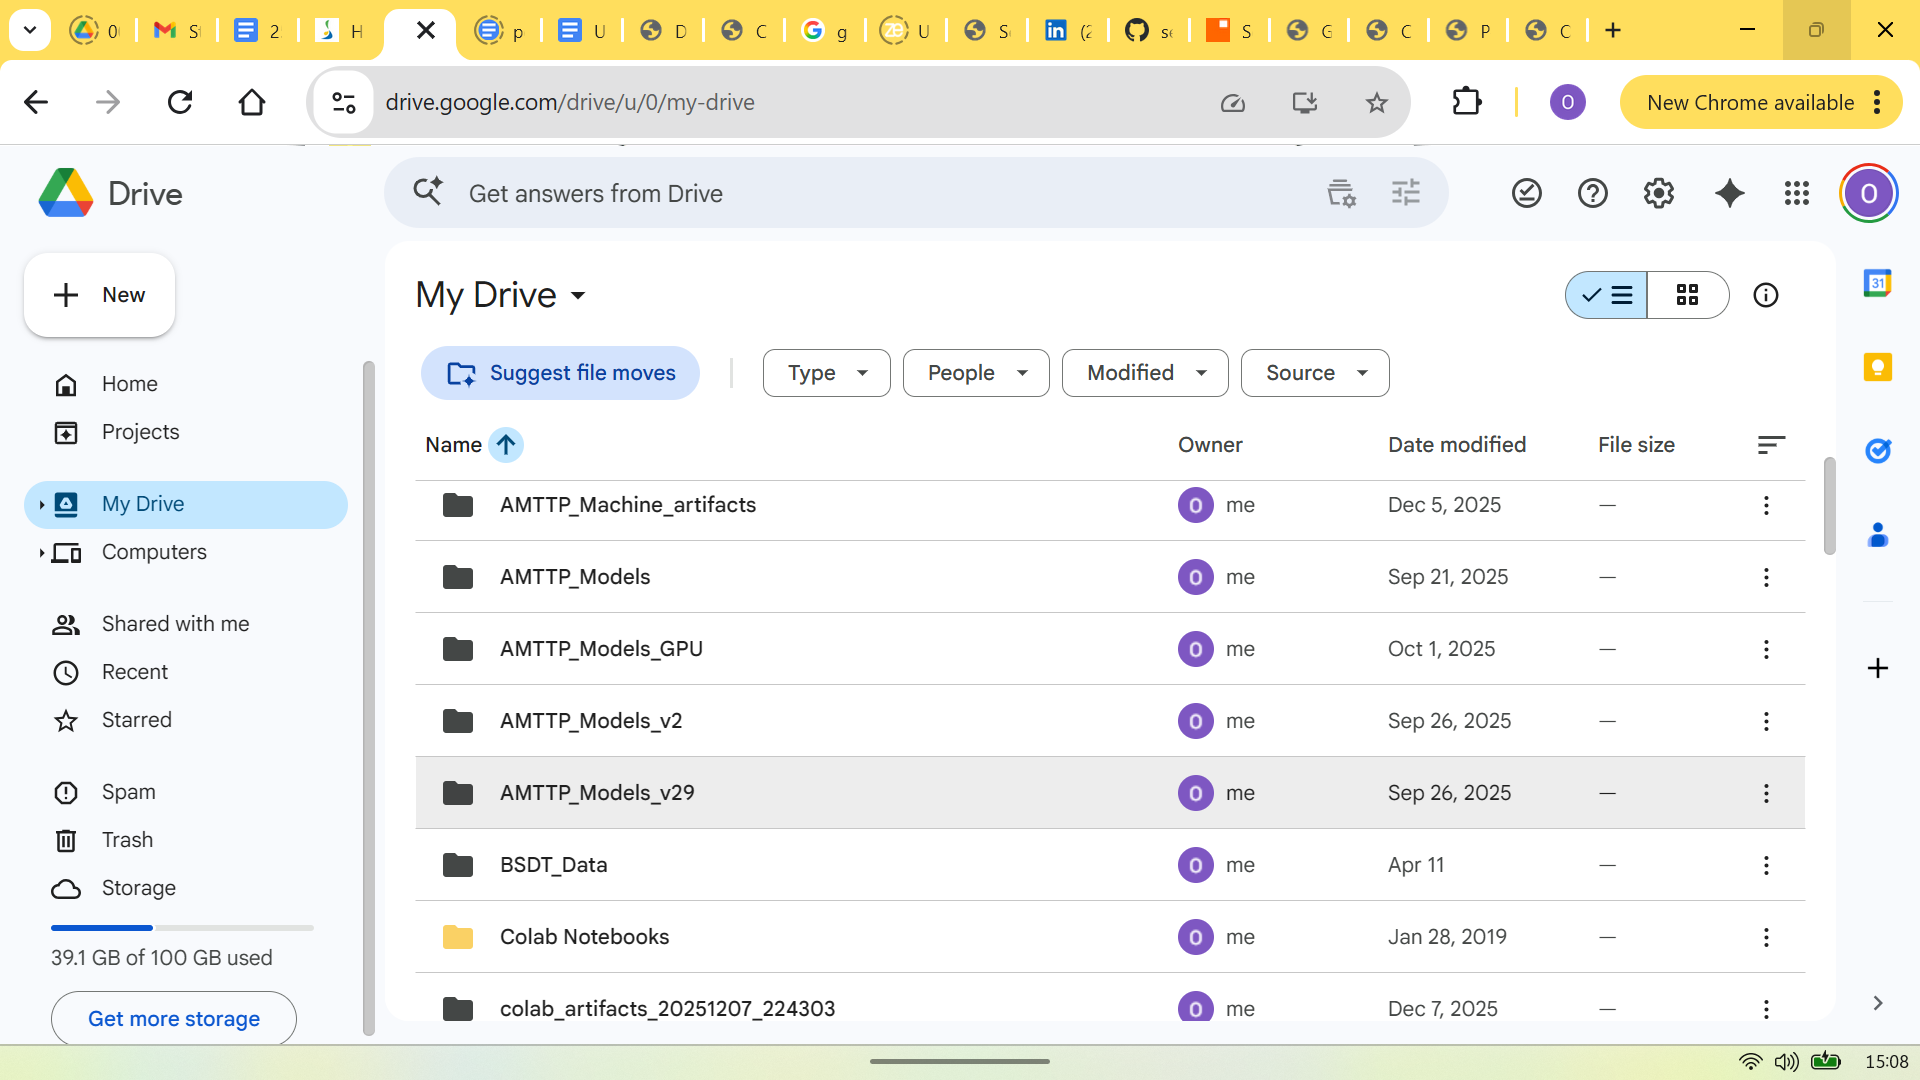
\includegraphics[width=0.93\textwidth]{images/google_drive_colab_artifacts.png}}
\end{center}
\vspace{0.1cm}

\noindent\textit{Figure 3: Google Drive listing (captured 13 May 2026) showing AMTTP ML artefact folders. Key entries: \textbf{AMTTP\_Machine\_artifacts} (Dec 5, 2025) and \textbf{colab\_artifacts\_20251207\_224303} (Dec 7, 2025) --- the folder name is an auto-generated ISO timestamp (7 Dec 2025, 22:43:03 UTC) from a Colab export script, confirming active model training outside the GitHub commit window. \textbf{AMTTP\_Models\_GPU} (Oct 1, 2025) and \textbf{AMTTP\_Models\_v2/\_v29} (Sep 26, 2025) show iterative ML versioning began at project inception, with artefacts integrated into the repository from January 2026 onwards.}

\end{document}